\section{The \bil Language}
\label{vine:language}


\begin{table}
\centering
\begin{tabular}{lll}
  \emphkind{program}&::=&
        \emphkind{stmt}*\\

  \emphkind{stmt}&::=&  
         \emphkind{var} := \emphkind{exp}
     $|$ {\tt jmp}(\emphkind{exp})
     $|$ {\tt cjmp}(\emphkind{exp},\emphkind{exp},\emphkind{exp})\\
     &&$|$ {\tt halt}(\emphkind{exp})
     $|$ {\tt assert}(\emphkind{exp})
     $|$ {\tt label} \emphkind{label\_kind}
     $|$ {\tt special}(string)\\

  \emphkind{exp}&::=& 
         {\tt load}(\emphkind{exp}, \emphkind{exp}, \emphkind{exp},
         \emphkind{$\tau_{\text{reg}}$})
        $|$ {\tt store}(\emphkind{exp}, \emphkind{exp},
        \emphkind{exp},\emphkind{exp},$\tau_{\text{reg}}$ )
     $|$ \emphkind{exp} $\Diamond_b$ \emphkind{exp}
     \\
     & & 
     $|$ $\Diamond_u$ \emphkind{exp}
     $|$ \emphkind{var}
     $|$ {\tt lab}(string)
     $|$ \emphkind{integer}
     $|$ {\tt
       cast}(\emphkind{cast\_kind},$\tau_{\text{reg}}$,\emphkind{exp})
\\
     & & $|$ {\tt let} \emphkind{var} {\tt =} \emphkind{exp} {\tt in} \emphkind{exp}
    
     $|$ {\tt unknown}(string, $\tau$)
     $|$ {\tt name}(\emphkind{exp})
     \\

  \emphkind{label\_kind}&::=&  \emphkind{integer} $|$ string \\
     
  \emphkind{cast\_kind}&::=&  
     {\tt unsigned}
     $|$ {\tt signed}
     $|$ {\tt high} 
     $|$ {\tt low}\\

%   \emphkind{decl}&::=& 
%          {\tt var} \emphkind{var}\\


  \emphkind{var}&::=& 
         (string, id$_v$, $\tau$)\\

  $\Diamond_b$&::=&
     $+ , - , * ,  /, /_s , \bmod , \bmod_s , \ll, \gg, \gg_a ,  \&,
        |, \xor, ==, !=, <, \leq , <_s, \leq_s$\\

  $\Diamond_u$&::=& $-$ (unary minus), $\sim$ (bit-wise not)\\

  \emphkind{value}&::=&  \emphkind{integer}
       $|$ \emphkind{memory} 
       $|$ string
       $|$ $\perp$  \\

  \emphkind{integer}&::=&          $n$ (:$\tau_{\text{reg}})$ \\


  \emphkind{memory}&::=&
        \{ \emphkind{integer} $\rightarrow$ \emphkind{integer}, 
             \emphkind{integer} $\rightarrow$ \emphkind{integer},
             \ldots \} (:$\tau_{\text{mem}}$) \\

  \emphkind{$\tau$} &::=&
          \emphkind{$\tau_{\text{reg}}$} 
      $|$ \emphkind{$\tau_{\text{mem}}$}\\

  \emphkind{$\tau_{\text{mem}}$} &::=& {\tt mem\_t}($\tau_{\text{reg}}$)
  $|$ {\tt array\_t}($\tau_{\text{reg}}, \tau_{\text{reg}}$)\\\
  
  \emphkind{$\tau_{\text{ reg}}$}&::=&
         {\tt reg1\_t} 
      $|$ {\tt reg8\_t} 
      $|$ {\tt reg16\_t} 
      $|$ {\tt reg32\_t} 
      $|$ {\tt reg64\_t}\\



\end{tabular}
\caption{The Binary Intermediate Language. Note commas separte
  operators.}
\label{vine:syntax}
\end{table}



Table~\ref{vine:syntax} shows the syntax of \bil. We use the term
``instruction'' to refer to an assembly-level instruction, and the
term ``statement'' to refer to instructions within \bil.  Thus, \bap
raises instructions to statements in \bil.  In \ref{vinesec:typecheck}
we give basic type-checking rules which disallow certain syntactically
valid but nonsensical expressions, and in ~\ref{vine:operational} we
provide the operational semantics. In the remainder of this section we
give an informal description and motivation for constructs in the IL.


\subsection{Values and Types}
The base types $\tau_{\text{reg}}$ in \bil IL are 1, 8, 16, 32, and
64-bit registers (i.e., $n$-bit vectors), and memories. Memories are
given type ${\tt mem\_t}(\tau_{\text{reg}})$, where $\tau_{\text{reg}}$
determines the type for memory addresses. For example, ${\tt
  mem}(\tau_{\text{reg32\_t}})$ corresponds to memory on a typical
32-bit machine.  

We also have arrays, which are given type ${\tt
  array\_t}(\tau_{\text{reg}},\tau_{\text{reg}})$. The tuple
$(\tau_{\text{reg}},\tau_{\text{reg}})$ specifies the index and
element type of an array, respectively.  As we will see, we use arrays
to \emph{normalize} endianed memory accesses.

There are three types of values in \bil. First, \bil has numbers $n$
of type $\tau_{\text{reg}}$. Second, \bil has memory values $\{
n_{a1} \rightarrow n_{v1}, n_{a2} \rightarrow n_{v2}, ... \}$, where
$n_{ai}$ denotes a number used as an address, and $n_{vi}$ denotes the
value stored at the address.  Finally, \bil has a nonsense value
$\perp$. $\perp$ values are not exposed to the user and cannot be
constructed in the presentation language.  $\perp$ is used internally
to indicate a failed execution.


\subsection{Expressions}
Expressions in \bil are side-effect free, and are similar to those
found in most languages.  \bil has binary operations $\Diamond_b$
(note ``\&'' and ``$|$'' are bit-wise), unary operations $\Diamond_u$,
constants, {\tt let} bindings, and casting.  Casting is used when
indexing registers under different addressing modes. For example, the
lower 8 bits of {\tt eax} in x86 are known as {\tt al}.  When lifting
x86 instructions, we use casting to project out the lower-bits of the
corresponding {\tt eax} register variable to an {\tt al} register
variable when {\tt al} is accessed.

The semantics of ${\tt load}(e_1, e_2, e_3, \tau_{\text{reg}})$ is to
load from the memory specified by $e_1$ at address $e_2$. In C, this
would loosely be written $e_1[e_2]$.  The parameter $e_3$ tells us the
endianness to use when loading bytes from memory. $e_3$ is forced to
be of type bool, where we arbitrary affix the meaning that 0 is little
endian and 1 is big endian (since 0 is ``littler'' than 1). Some
architecture consistently use the same endianness, e.g., for x86, the
value of $e_3$ will always correspond to little-endianness.  However,
other architectures such as ARM specify the endianness of a load at
run-time.  Finally, $\tau_{\text{reg}}$ tells us how many bytes to
load.  In C, if $e_1$ is of type $\tau$, then $e_1[e_2]$ loads {\tt
  sizeof($\tau$)} bytes.  $\tau_{\text{reg}}$ similarly tells us how
many bytes to load from memory. While technically we could infer
$\tau_{\text{reg}}$ given $e_1$, we keep it in the IL explicitly for
efficiency.


In \bil, the {\tt store} operation is pure (i.e., side-effect
free). The advantage of pure memory operations in \bil notation is it
makes it possible to syntactically distinguish what memory is modified
or read.  One place we take advantage of this is in SSA
(see~\ref{vine:backend}) where both scalars and memory have a unique
single static assignment location.

Each {\tt store} expression must specify what memory to load or store
from.  The resulting memory is returned as a value.  The semantics of
${\tt store}(e_1, e_2, e_3, e_4, \tau_{\text{reg}})$ are to store in
memory $e_1$, starting at address $e_2$ the value $e_3$.  The store is
performed given the endianness of $e_4$.  This may seem very
complicated when reading. However, the operational semantics are quite
simple: you may want to read the  {\sc store} rules.


The last expression type of note is {\tt unknown}.  An {\tt unknown}
specifies an operation we could not lift to \bil.  The purpose of an
unknown is to adhere to the \bap principle to \emph{know what you do
  not know}.  Consider the case where Intel adds a new instruction,
e.g., as happens in each processor revision.  \bap may not know about
such instructions, thus cannot raise it to \bil. One option would be
to ignore such instructions. However, the result of any analysis would
be suspect in this case. A sound option is to abort lifting and raise
an error. However, we often end up not interested in particular
instructions. Our solution is to raise such instructions, when
possible, to an assignment (where the left hand side is of the correct
type and name) with the actual operation left unspecified as {\tt
  unknown}.

\subsection{Statements and Programs}

A program in \bil is a sequence of statements.  There are 7 different
kinds of instructions. The language has assignments, jumps,
conditional jumps, and labels.  The target of all jumps and
conditional jumps must be a valid label in our operational semantics,
else the program terminates in the error state ($\perp$).  Note that a
jump to an undefined location (e.g., a location that was not
disassembled such as to dynamically generated code) results in the
\bap program halting with $\perp$ (see~\ref{vine:operational}). A
program can halt normally at any time by issuing the {\tt halt}
statement.  We also provide {\tt assert}, which acts similar to a C
assert: the asserted expression must be true, else the machine halts
with $\perp$.

A {\tt special} in \bil corresponds to a call to an externally
defined procedure or function. {\tt special} statements typically
arise from system calls.  The {\tt id} of a {\tt special} indexes the
kind of special, e.g., what system call.

The semantics of {\tt special} are up to the analysis; its operational
semantics are not defined (Chapter~\ref{vine:operational}).  We
include {\tt special} as an instruction type to explicitly distinguish
calls that alter the soundness of an analysis. A typical approach to
dealing with {\tt special} is to replace {\tt special} with an
analysis-specific summary function written in the \bap IL that is
appropriate for the analysis.


\begin{figure}

\subfloat[][]{
\begin{minipage}[b]{2.5in}
\begin{footnotesize}
\begin{tightcode}
// x86 instr dst,src\newline
1. mov [eax], 0xaabbccdd\newline
2. mov ebx, eax\newline
3. add ebx, 0x3\newline
4. mov eax, 0x1122\newline
5. mov [ebx], ax\newline
6. sub ebx, 1\newline
7. mov ax, [ebx]\newline
\end{tightcode}
\end{footnotesize}
\end{minipage}
\label{endian:code}
}
%\begin{minipage}[c]{5in}
%\begin{subfigure}
\subfloat[][]{
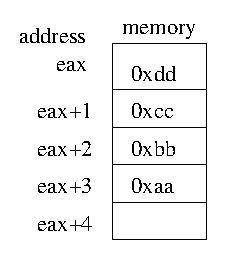
\includegraphics[scale=.7]{fig/memvsarray-1}
\label{endian:membefore}
}
\subfloat[][]{
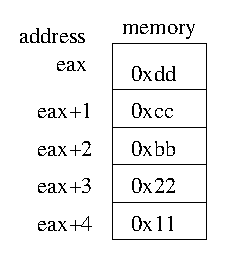
\includegraphics[scale=.7]{fig/memvsarray-2}
\label{endian:memafter}
}
%\end{subfigure}
%\end{minipage}
\caption{(a) shows an example of little-endian stores as found in x86 that
  partially overlap. (b) shows memory after executing line 1, and (c)
  shows memory after executing line 5. Line 7 will load the value 0x22bb.}
\label{fig:endian}
\end{figure}

\section{Normalized Memory} 
\label{vine:normalized}

The endianness of a machine is usually specified by the byte-ordering
of the hardware.  Little endian architectures such as x86 put the
low-order byte first. Big-endian architecture put the high-order byte
first. Some architectures, such as ARM, allow the endianness to be
specified by the instruction, e.g., {\tt mov} would take three
arguments: the source, destination, and endianness for which to
perform the move.


We must take endianness into account when analyzing memory
accesses. Consider the assembly in Figure~\ref{endian:code}. The {\tt
  mov} operation on line 2 writes 4 bytes to memory in little endian
order (since x86 is little endian). After executing line 2, the
address given by {\tt eax} contains byte {\tt 0xdd}, {\tt eax+1}
contains byte {\tt 0xcc}, and so on, as shown in
Figure~\ref{endian:membefore}. Lines 2 and 3 set {\tt ebx =
  eax+2}. Line 4 and 5 write the 16-bit value {\tt 0x1122} to {\tt
  ebx}.  An analysis of these few lines of code needs to consider that
the write on line 4 overwrites the last byte written on line 1, as
shown in Figure~\ref{endian:memafter}. Considering such cases requires
additional logic in each analysis. For example, the value loaded on
line 7 will contain one byte from each of the two stores.

%  In normalized memory,
% all addresses are of the same type $\tau_{\text{addr}} \in
% \tau_{\text{reg}}$, and all values are of type {\tt reg8\_t}.

\begin{figure}
\begin{footnotesize}
\begin{code}  
1. mem4 = let mem1 = store(mem0,eax, 0xdd, 0, reg8\_t) in 
           let mem2 = store(mem1, eax+1, 0xcc, 0, reg8\_t) in 
           let mem3 = store(mem2, eax+2, 0xbb, 0, reg8\_t) in 
               store(mem3, eax+3, 0xcc, 0, reg8\_t);
...
5. mem6 = let mem5 = store(mem4, ebx, 0x22, 0, reg8\_t) in 
             store(mem5, ebx+1, 0x22, 0, reg8\_t) 
...
7. value = let b1 = load(mem6, ebx, 0, reg8\_t) in
            let b2 = load(mem6, ebx+1, 0, reg8\_t) in 
            let b1' = cast(unsigned, b1, 0, reg16\_t) in 
            let b2' = cast(unsigned, b2, 0, reg16\_t) in 
               (b2' $\ll$ 8) $|$ b1';
\end{code}
\end{footnotesize}
\caption{Normalized version of the store and load from Figure~\ref{endian:code}.}
\label{endian:normalized}
\end{figure}


We say a memory is \emph{normalized} for a $b$-byte addressable memory
if all loads and stores are exactly $b$-bytes and $b$-byte
aligned. In x86, memory is byte addressable, so a
normalized memory for x86 has all loads and stores at the byte
level. The normalized form for the write on Line 1 of
Figure~\ref{endian:code} in \bil is shown in
Figure~\ref{endian:normalized}.  Note that the subsequent load on line 7
is with respect to the current memory {\tt mem6}.

Normalized memory makes writing program analyses involving memory
easier.  Analysis is easier because normalized memory syntactically
exposes memory updates that are otherwise implicitly defined by the
endianness.  As a result, analyses do not have to reason explicitly
about overlapping memory, byte order, etc. \bap provides utilities for
normalizing all memory operations so that users can write analysis
more easily.



% Endianness can complicate analysis. 
% specified bit-ordering of the hardware, i.e., a specification of which
% hardware bit corresponds to the low-order bit in a number. 

% Assembly memory operations are
% performed with respect to the endianness (byte ordering) of the
% hardware. 

% A memory operation may either be little endian or big
% endian. A little endian operation to address $a$ stores the low-order
% byte in a register in the lowest memory address, the next lowest-order
% byte in the



% We provide routines to conver little and big endian memories to
% normalized form. The advantage of normalized memory is it eases
% analysis.  For example, consider the x86 instruction sequence shown
% in Figure~\ref{fig:memvsarray}.

% Instruction 1 stores the value 0xaabbccdd into the address given by
% {\tt \%eax}. Since x86 is little-endian, the bytes are stored in
% memory from lowest to highest, as shown in Figure~\ref{fig:}.

% which stores the value in the 4-byte {\tt \%ebx} register
% into the address given by {\tt \%eax}. This instruction on x86 is
% syntatic sugar for storing the low-order byte of {\tt \%ebx} at
% address {\tt \%eax}, the second low-order byte in {\tt \%eax+1}, the
% third in {\tt \%eax+2}, and the high-order byte in {\tt \%eax+3}. In
% \bap, a normalized memory desugars such statements, so {\tt mov
%   *\%eax, \%ebx} becomes:
% \begin{footnotesize}
% \begin{code}
%   // mov *\%eax, \%ebx is desugared in normalized vine memory as
%     mem1 = store(mem0, eax,   ebx \& 0x000000ff);
%     mem2 = store(mem1, eax+1, ebx \& 0x0000ff00);
%     mem3 = store(mem2, eax+2, ebx \& 0x00ff0000);
%     mem4 = store(mem3, eax+3, ebx \& 0xff000000);
% \end{code}
% \end{footnotesize}


% Typically an assembly program works on a single memory.  

% Values in \bap are either register values or memories.  

% Scalar variables in \bap roughly correspond to registers. Although

% In this section we describe the \bap IL.  We first present the \bap
% IL.  In \bap, we have several statements that are derived
% forms. These derived forms are a ``syntatic sugar'' that make writing
% analysis easier, though add no real power to the language.  As
% mentioned, one of the principles of \bap is to treat assembly as a
% first class language. One consequence is \bap does not have
% functions. However, we have observed that several analysis benefit
% from assuming functions exist. We present \bap$_f$, which is an
% extension to \bap which includes functions.


